\chapter{Experimental Results}
\label{chapter6_experiments}
\thispagestyle{empty}

\vspace{0.5cm}

In this chapter we show experimental results of our algorithm on some Atari
games.
We show that the representation of the states learned by our feature extraction 
pipeline is suitable for the semi-batch control approach with FQI, and that 
our agent is able to learn non-trivial policies with good sample efficiency on 
different environments.

\section{Premise}
Our approach aims at optimizing sample efficiency, but does not account for
the computational complexity of training and evaluating the full pipeline. 
All three main components of the algorithm benefit a great deal from parallel 
computing, to the point where the hardware itself is a key component in 
making the algorithm treatable at all. 
We were thus strongly limited in our experimental phase by our access to 
hardware for heavy parallel computing, with even costs for renting servers on 
cloud providers being prohibitive when considering our runtime. 
We therefore had to be extremely selective in what experiments to run, each of 
which took days at a time, and well balanced between exploring new possibilities
(hyperparameters, network architectures, environments) and evaluating current 
configurations. 
In this chapter we report the best findings across all our experiments and we 
try to outline the thought process that led us to favor some choices over others.
The hardware configurations of the three servers that we used for experiments is
reported in Table \ref{t:servers}. 
%
\begin{table}
    \centering
    \begin{tabular}{c c c c} 
	\hline
	Server ID & vCPU count & GPU                          & RAM (GB) \\ 
	\hline 
	\#$1$     & $64$       & None                         & $252$ \\
	\#$2$     & $8$        & $1 \times$ Nvidia Tesla K40C & $32$ \\
	\#$3$     & $4$        & $1 \times$ Nvidia Tesla K40C & $32$ \\
	\hline
    \end{tabular}
    \caption[Server configurations for experiments]{Server configurations for 
	     experiments.}
    \label{t:servers}
\end{table}
%

The code implementation of the algorithm was based on Python 2.7 and its 
\textit{de facto} standard libraries for general machine learning, GPU-based 
deep learning, and linear algebra. 
We trained and used the AE on an \textit{Nvidia Tesla K40C} GPU, using the 
\textit{Keras 2.0.6} API as interface to the \textit{Tensorflow 1.3.0} library 
for deep learning, whereas the training and evaluation of Extra-Trees 
for RFS and FQI was run on CPU using the \textit{Scikit-Learn 0.19.0} library.
We used the implementations of FQI and RFS provided in the open source 
\textit{IFQI} library by Matteo Pirotta.
Finally data manipulation and any other algebraic operations were done with 
\textit{Numpy 1.13.1}.

\section{Baseline}\label{s:exp_baseline}
To evaluate the results of our approach with respect to other algorithms, we 
compared our agent's performance with that of DQN and of a fully random policy. 
For DQN, we used an open source implementation of the paper by Mnih et al.\ \cite{mnih2015human} 
with the same exact parametrization, and run the algorithm with a total of $50$ 
million online training samples on the \textit{Breakout, Pong}, and \textit{Space 
Invaders} environments from the Atari games (reported in Table \ref{t:envs_used}).
To remain loyal to the original DQN methodology, we run an evaluation phase 
of $125000$ steps every $250000$ collected training samples. A similar 
evaluation was also run once on the fully random policy.
%
\begin{table}
    \centering
    \begin{tabular}{l c c c c} 
	\hline
	Environment    & $|A|$ & Random   & Best DQN  & Samples for best DQN \\ 
	\hline 
	Breakout       & $4$   & $1.09$   & $319.83$  & $\approx19250000$ \\
	Pong           & $6$   & $-20.49$ & $19.82$   & $\approx35250000$ \\
	Space Invaders & $6$   & $174.46$ & $1125.41$ & $\approx31500000$ \\
	\hline
    \end{tabular}
    \caption[Performance of baseline algorithms]{Average performance of baseline
	     algorithms.}
    \label{t:envs_used}
\end{table}
%
We therefore defined three main indicators that we used for comparison, and for 
each environment we considered namely:
\begin{enumerate}
    \item the performance of the fully random policy during $125000$ evaluation
    steps, in order to determine the base learning threshold;
    \item the performance of DQN during $125000$ evaluation steps under an 
    $\varepsilon$-greedy policy with $\varepsilon = 0.05$;
    \item the number of training samples collected by DQN in order to reach the
    best performance.
\end{enumerate}
We used these performance indicators to define the score range in which our 
agent should be, and to compare the order of magnitudes of the numbers of 
samples required by our algorithm and DQN (which requires samples in the order 
of $10^7$ for all environments). 
To evaluate the performance of our baselines, we simply considered the average 
non-clipped cumulative reward across all evaluation episodes. 
The performance of the baseline algorithms is reported in Table \ref{t:envs_used} 
and Figures \ref{f:BO_baseline}, \ref{f:P_baseline} and \ref{f:SI_baseline}.
%
\begin{figure}
    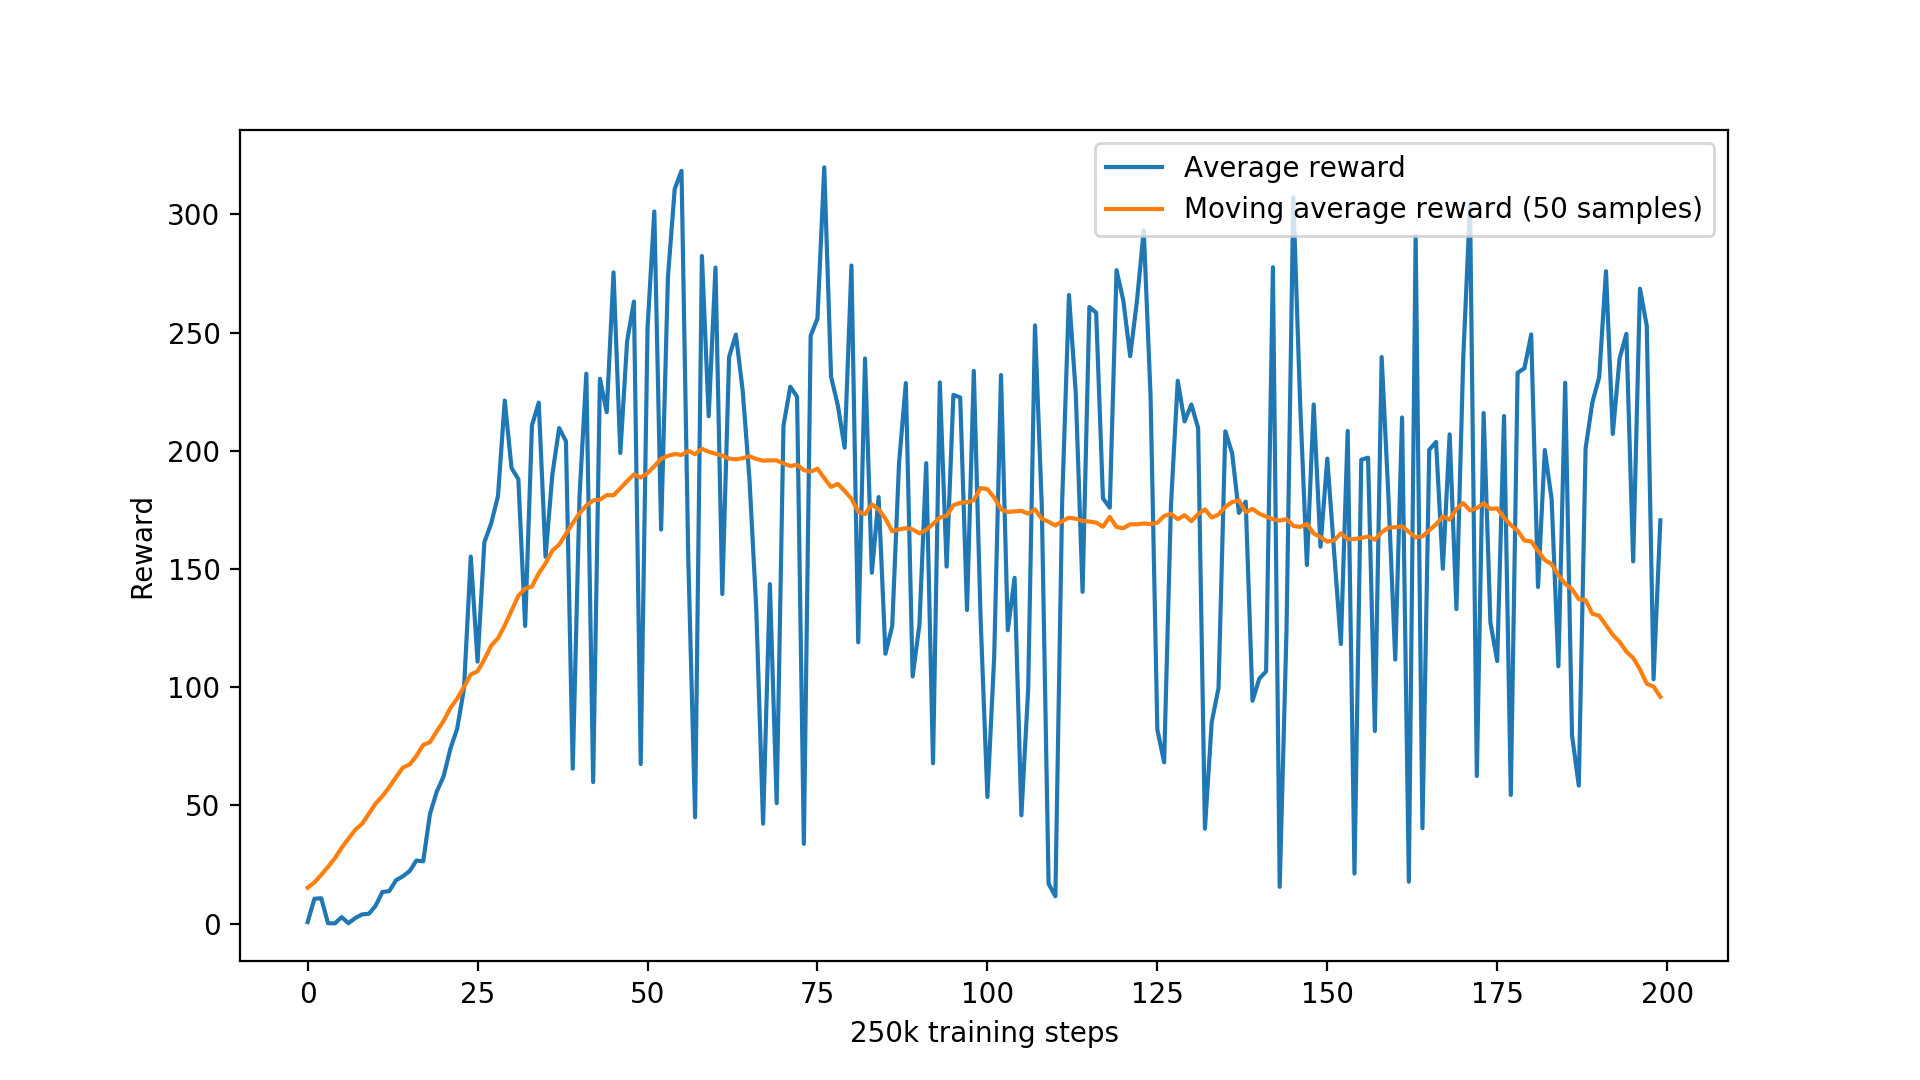
\includegraphics[width=\textwidth]{pictures/experiments/baseline_breakout}
    \centering
    \caption[Average performance of DQN in Breakout]{Average evaluation reward of 
	    DQN in Breakout, with the moving average of 50 consecutive evaluations 
	    highlighted to show the trend.}
    \label{f:BO_baseline}
\end{figure}
%
%
\begin{figure}
    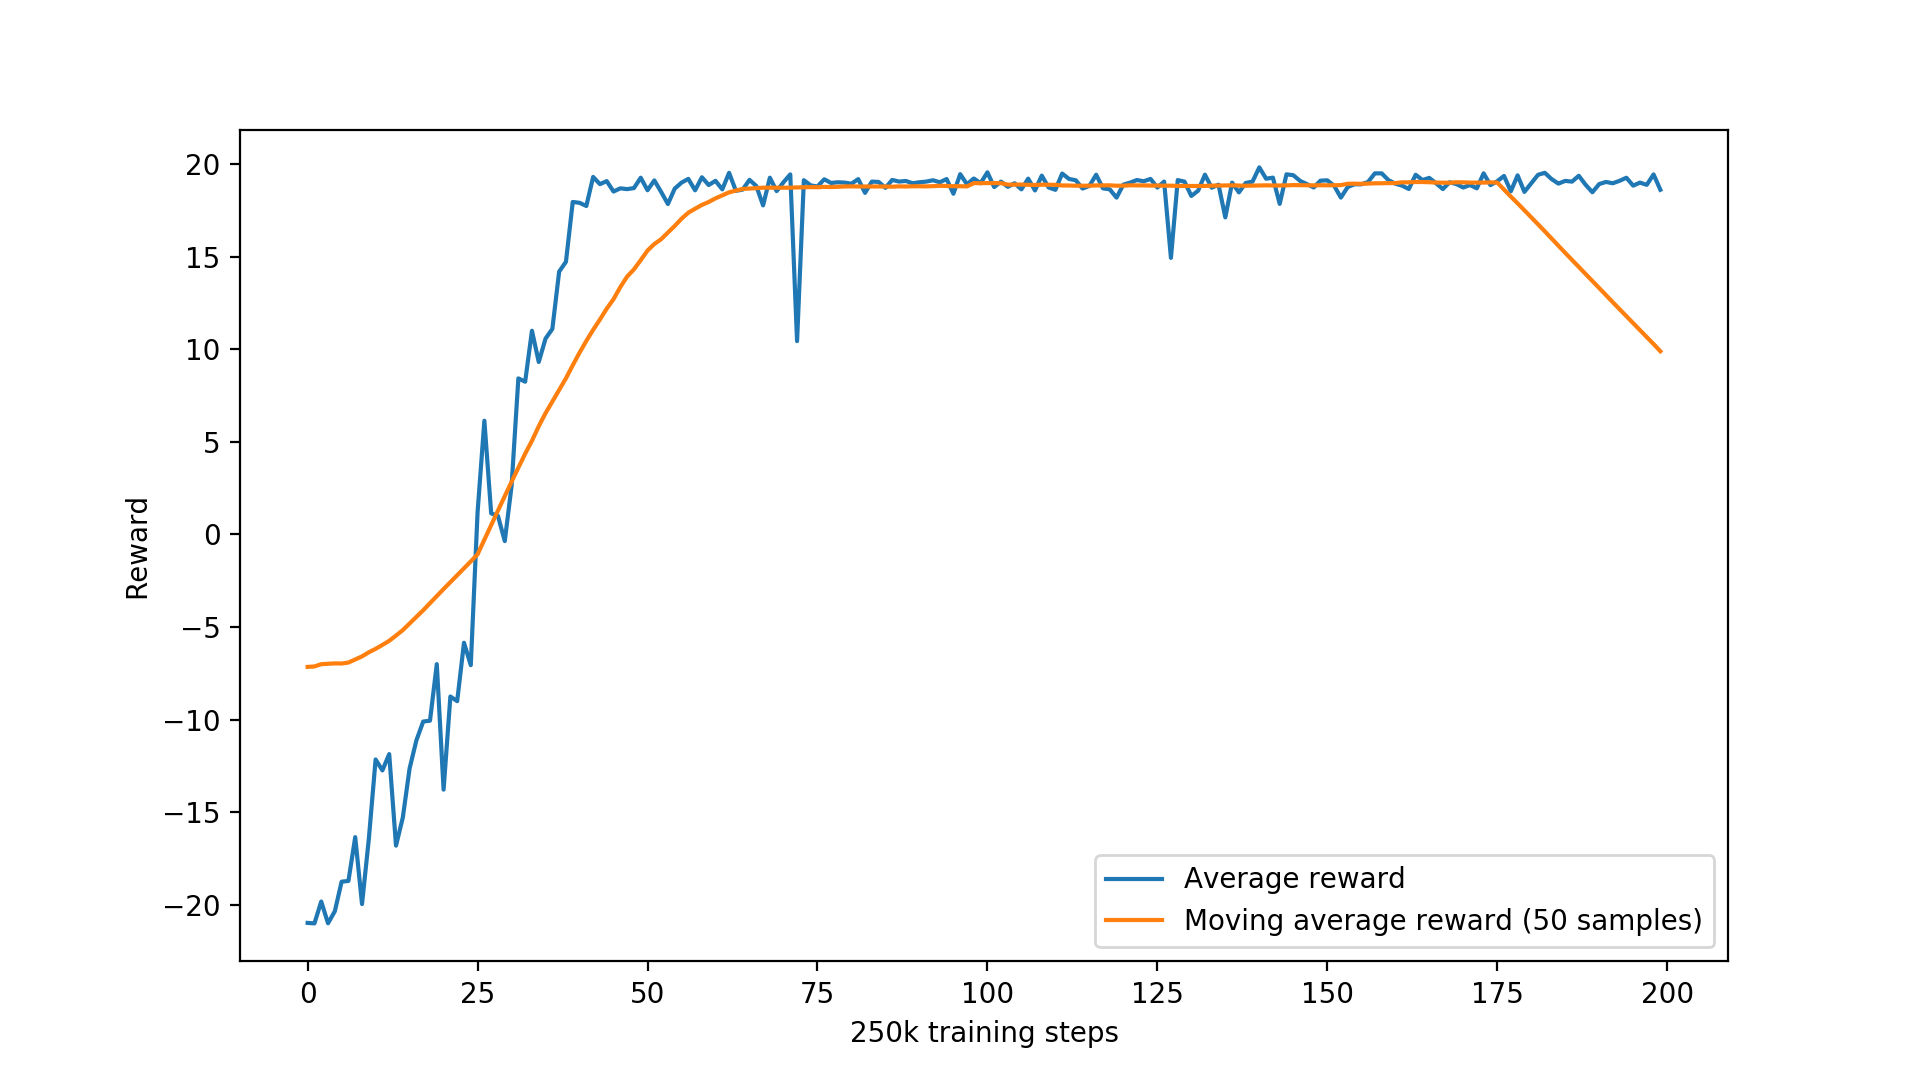
\includegraphics[width=\textwidth]{pictures/experiments/baseline_pong}
    \centering
    \caption[Average performance of DQN in Pong]{Average evaluation reward of DQN in
	    Pong, with the moving average of 50 consecutive evaluations highlighted
	    to show the trend.}
    \label{f:P_baseline}
\end{figure}
%
%
\begin{figure}
    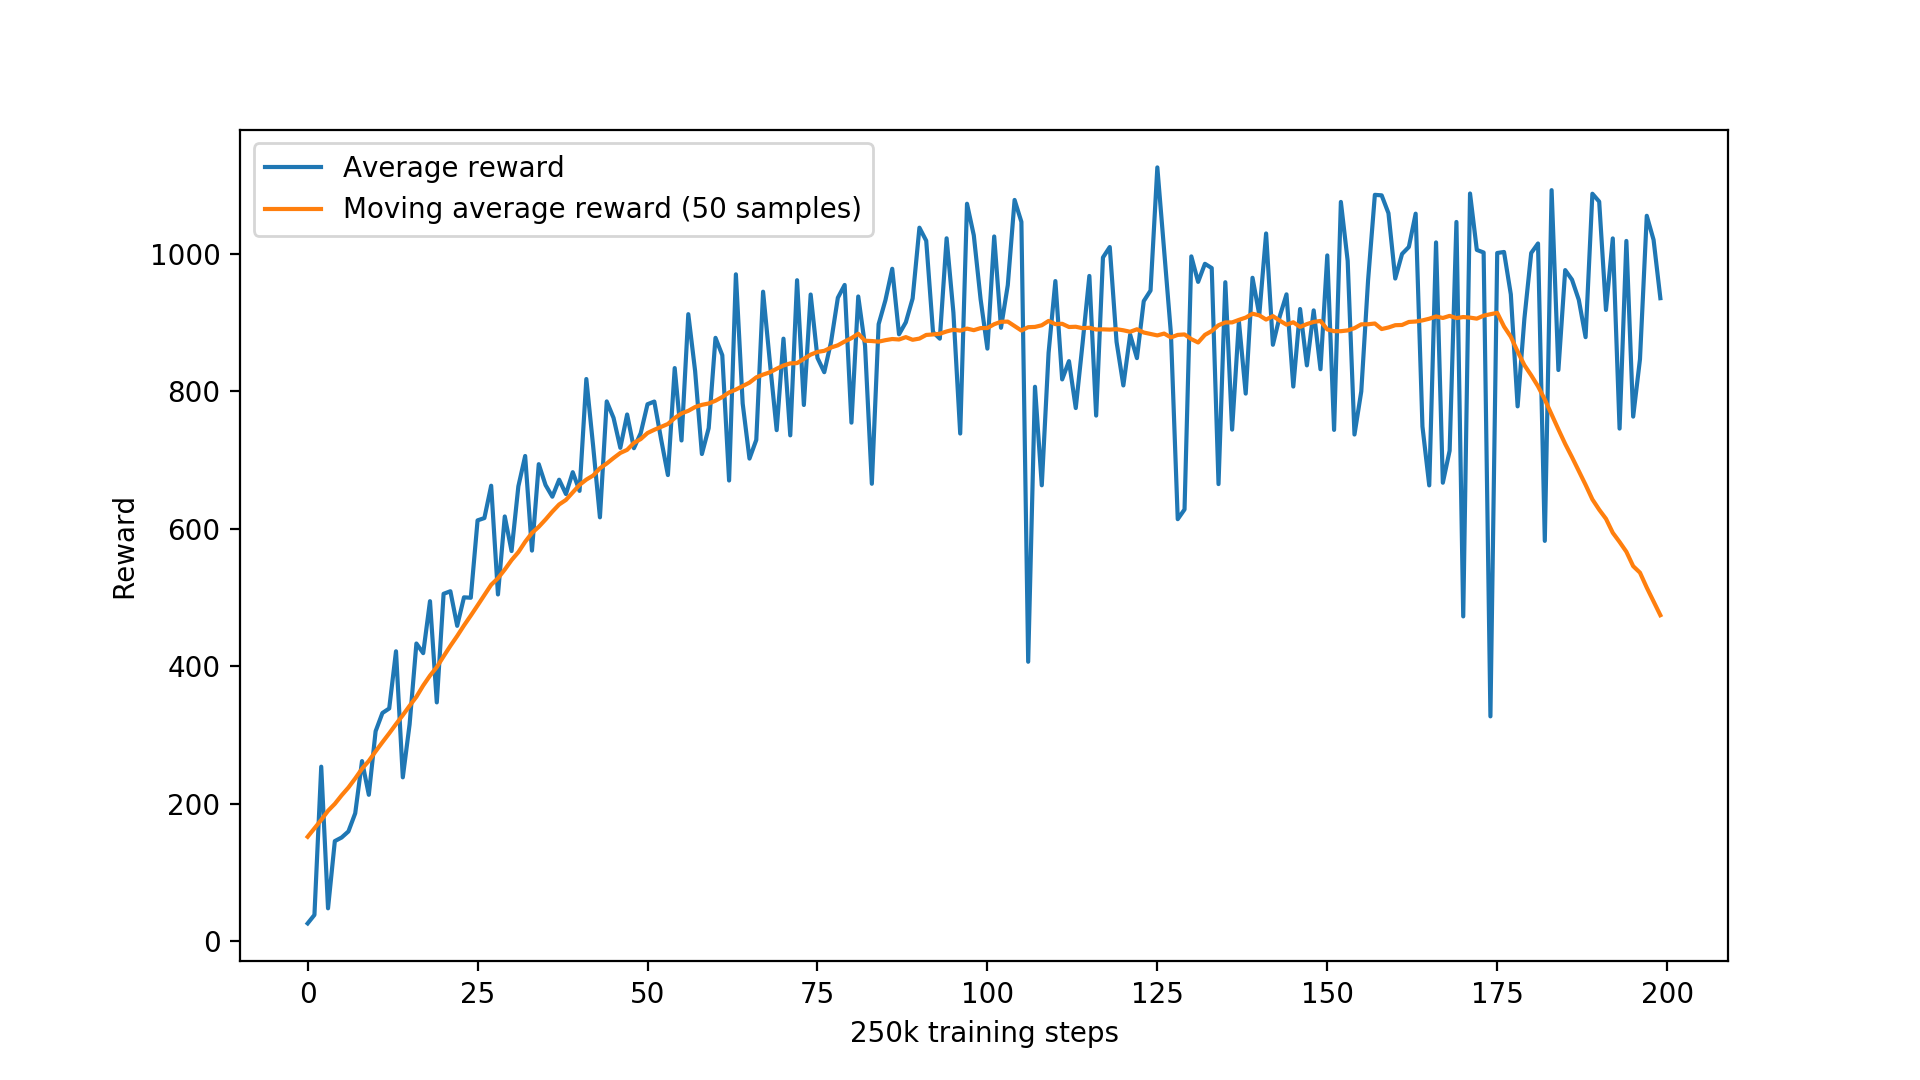
\includegraphics[width=\textwidth]{pictures/experiments/baseline_space_invaders}
    \centering
    \caption[Average performance of DQN in Space Invaders]{Average evaluation reward
	    of DQN in Space Invaders, with the moving average of 50 consecutive 
	    evaluations highlighted to show the trend.}
    \label{f:SI_baseline}
\end{figure}
%

\section{Autoencoder}
Due to the extremely high training and (especially) evaluation times that we 
encountered in FQI\footnote{Slow performance in evaluation is due to the 
sample-wise forward prediction across the full pipeline required at each step
of evaluation episodes. Specifically, each prediction of the $Q$ function needs 
a forward pass of the 4-layer encoder (which requires loading data in the GPU)
and a forward pass of Extra-Trees (which due to an internal inefficiency in 
\textit{Scikit-learn} was extremely slow when predicting on a single sample).},
and the almost intractable runtime of RFS\footnote{Which can take more than a 
week to complete, on our most performing server.}, we had to formally assess the 
suitability of the extracted features for control problems before moving on to 
train the other components in the pipeline. 
To do so, we run a series of tests devised to highlight different aspects of
the feature extraction. Once a training configuration was deemed satisfactory, 
we kept it fixed for all the following experiments.
%
\begin{figure}
    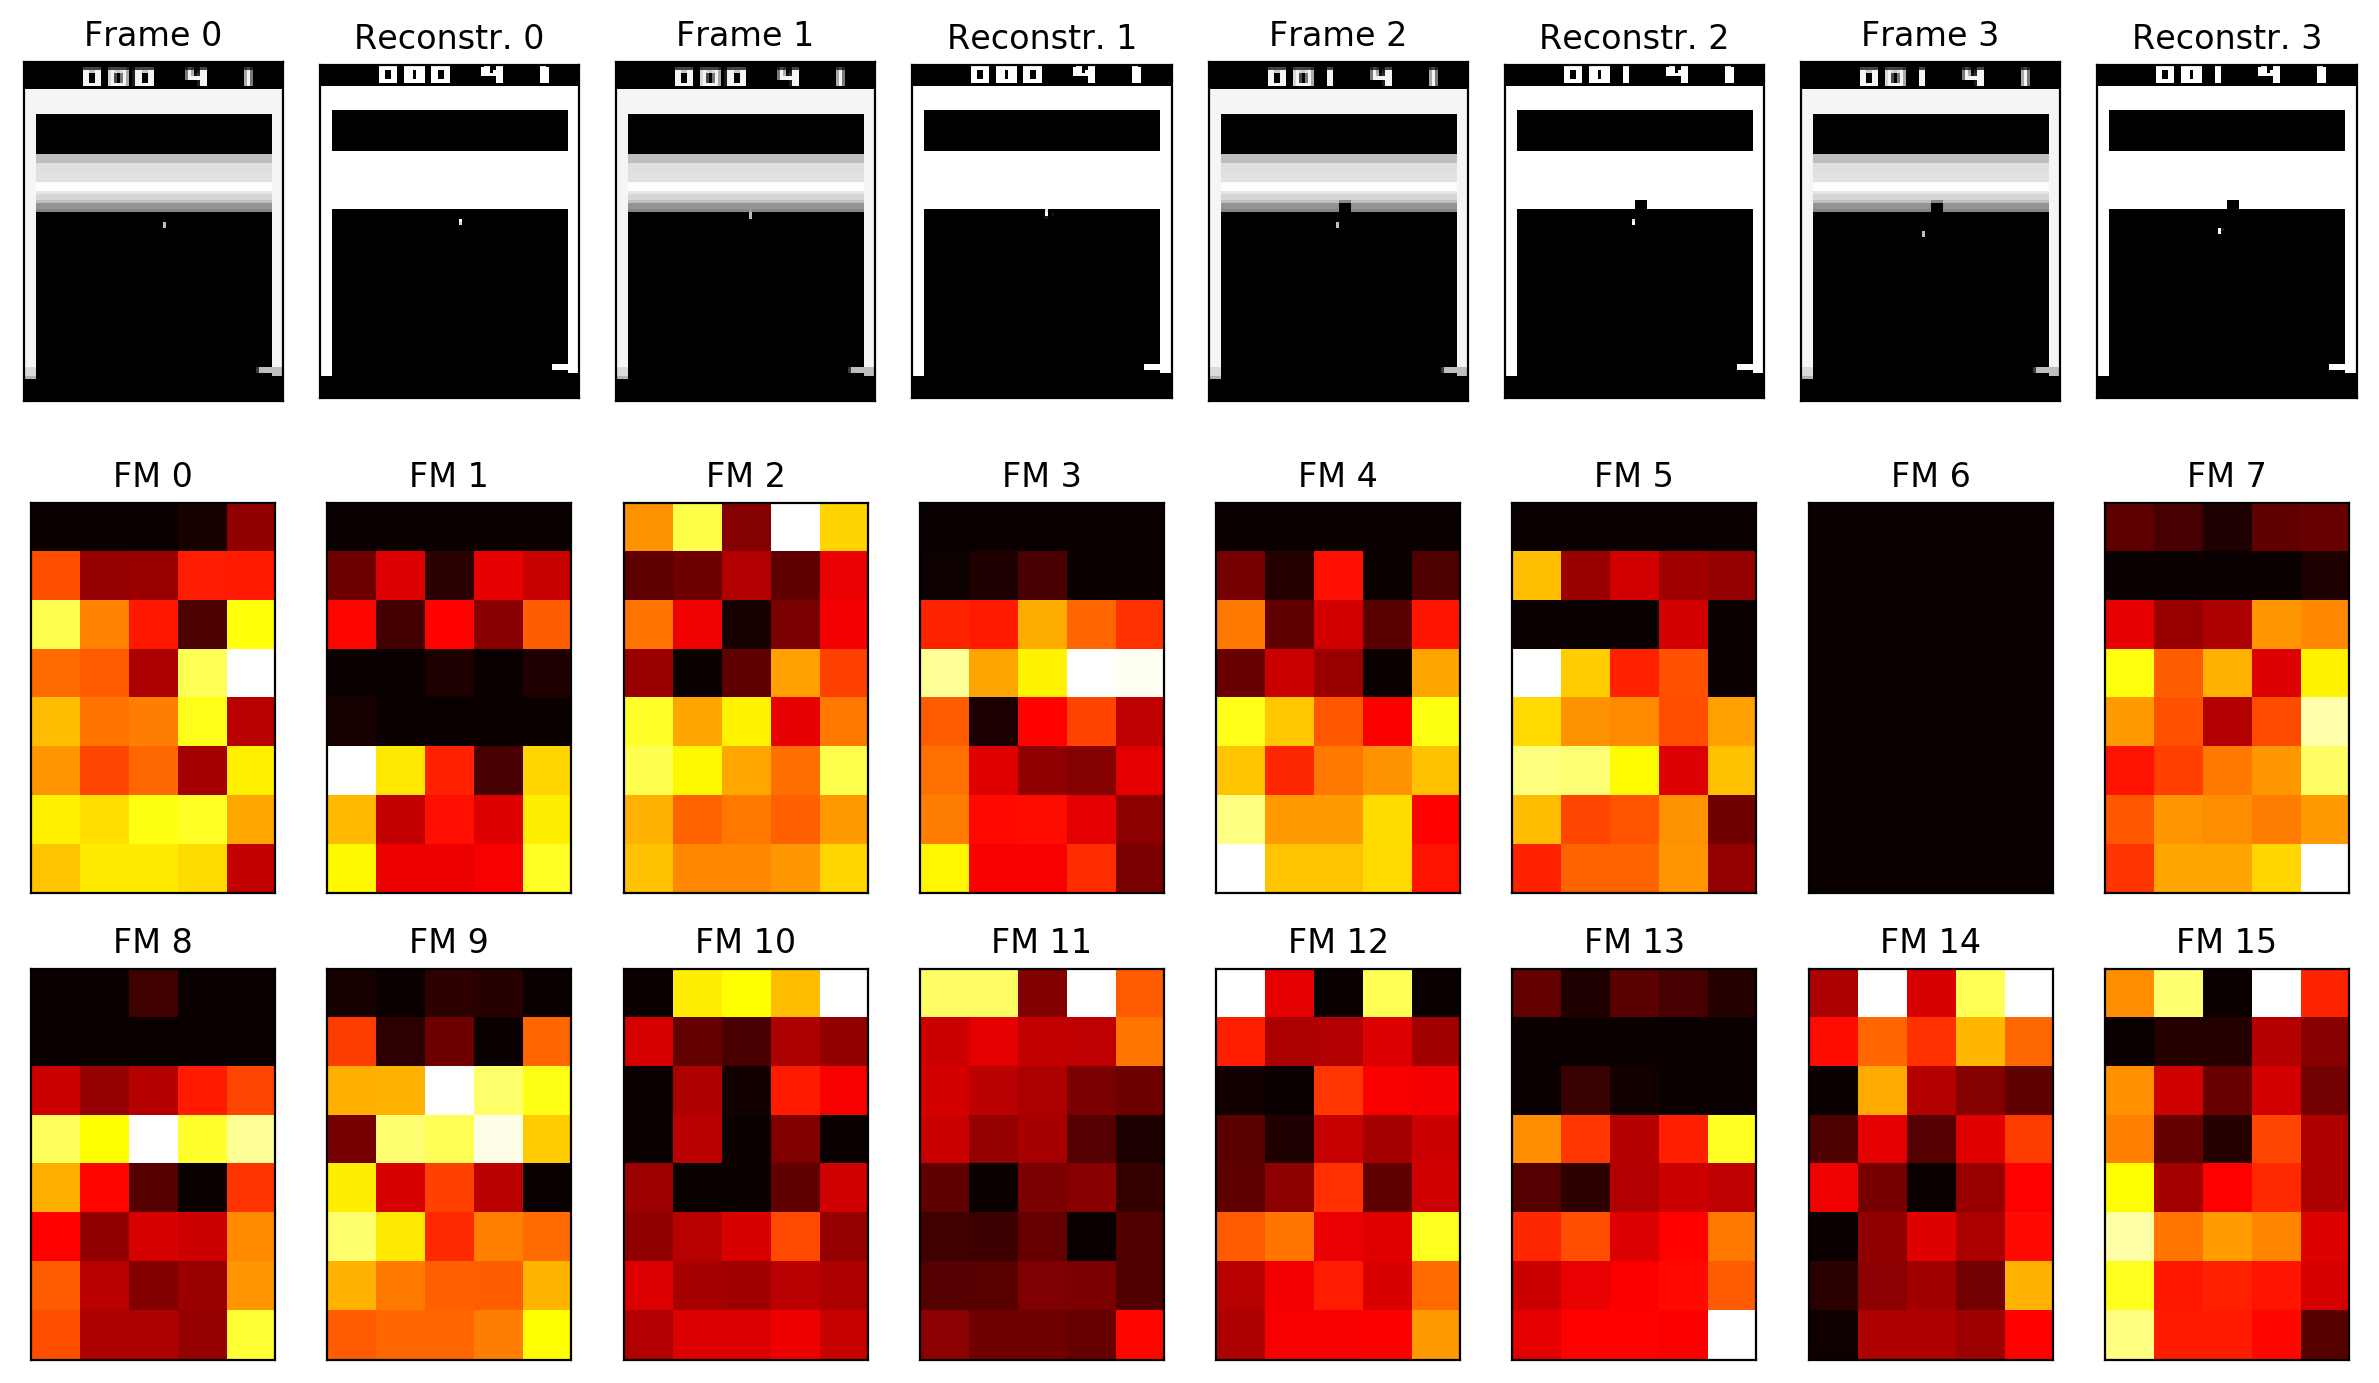
\includegraphics[width=\textwidth]{pictures/experiments/reconstr_breakout}
    \centering
    \caption[AE reconstruction and feature maps on Breakout]{AE reconstruction 
    and feature maps on Breakout. 
    Each pair in the top row shows a frame of a $4$-channel state $s$ given as input 
    to the AE, with its associated 
    reconstructed channel. The bottom two rows show the relative activation values 
    of the innermost feature maps before the flatten layer, after encoding $s$: 
    colors represent a heatmap from black ($0$) to white (map-wise maximum 
    activation value). The same applies to Figures \ref{f:P_reconstr} and 
    \ref{f:BO_reconstr}.}
    \label{f:BO_reconstr}
\end{figure}
%
%
\begin{figure}
    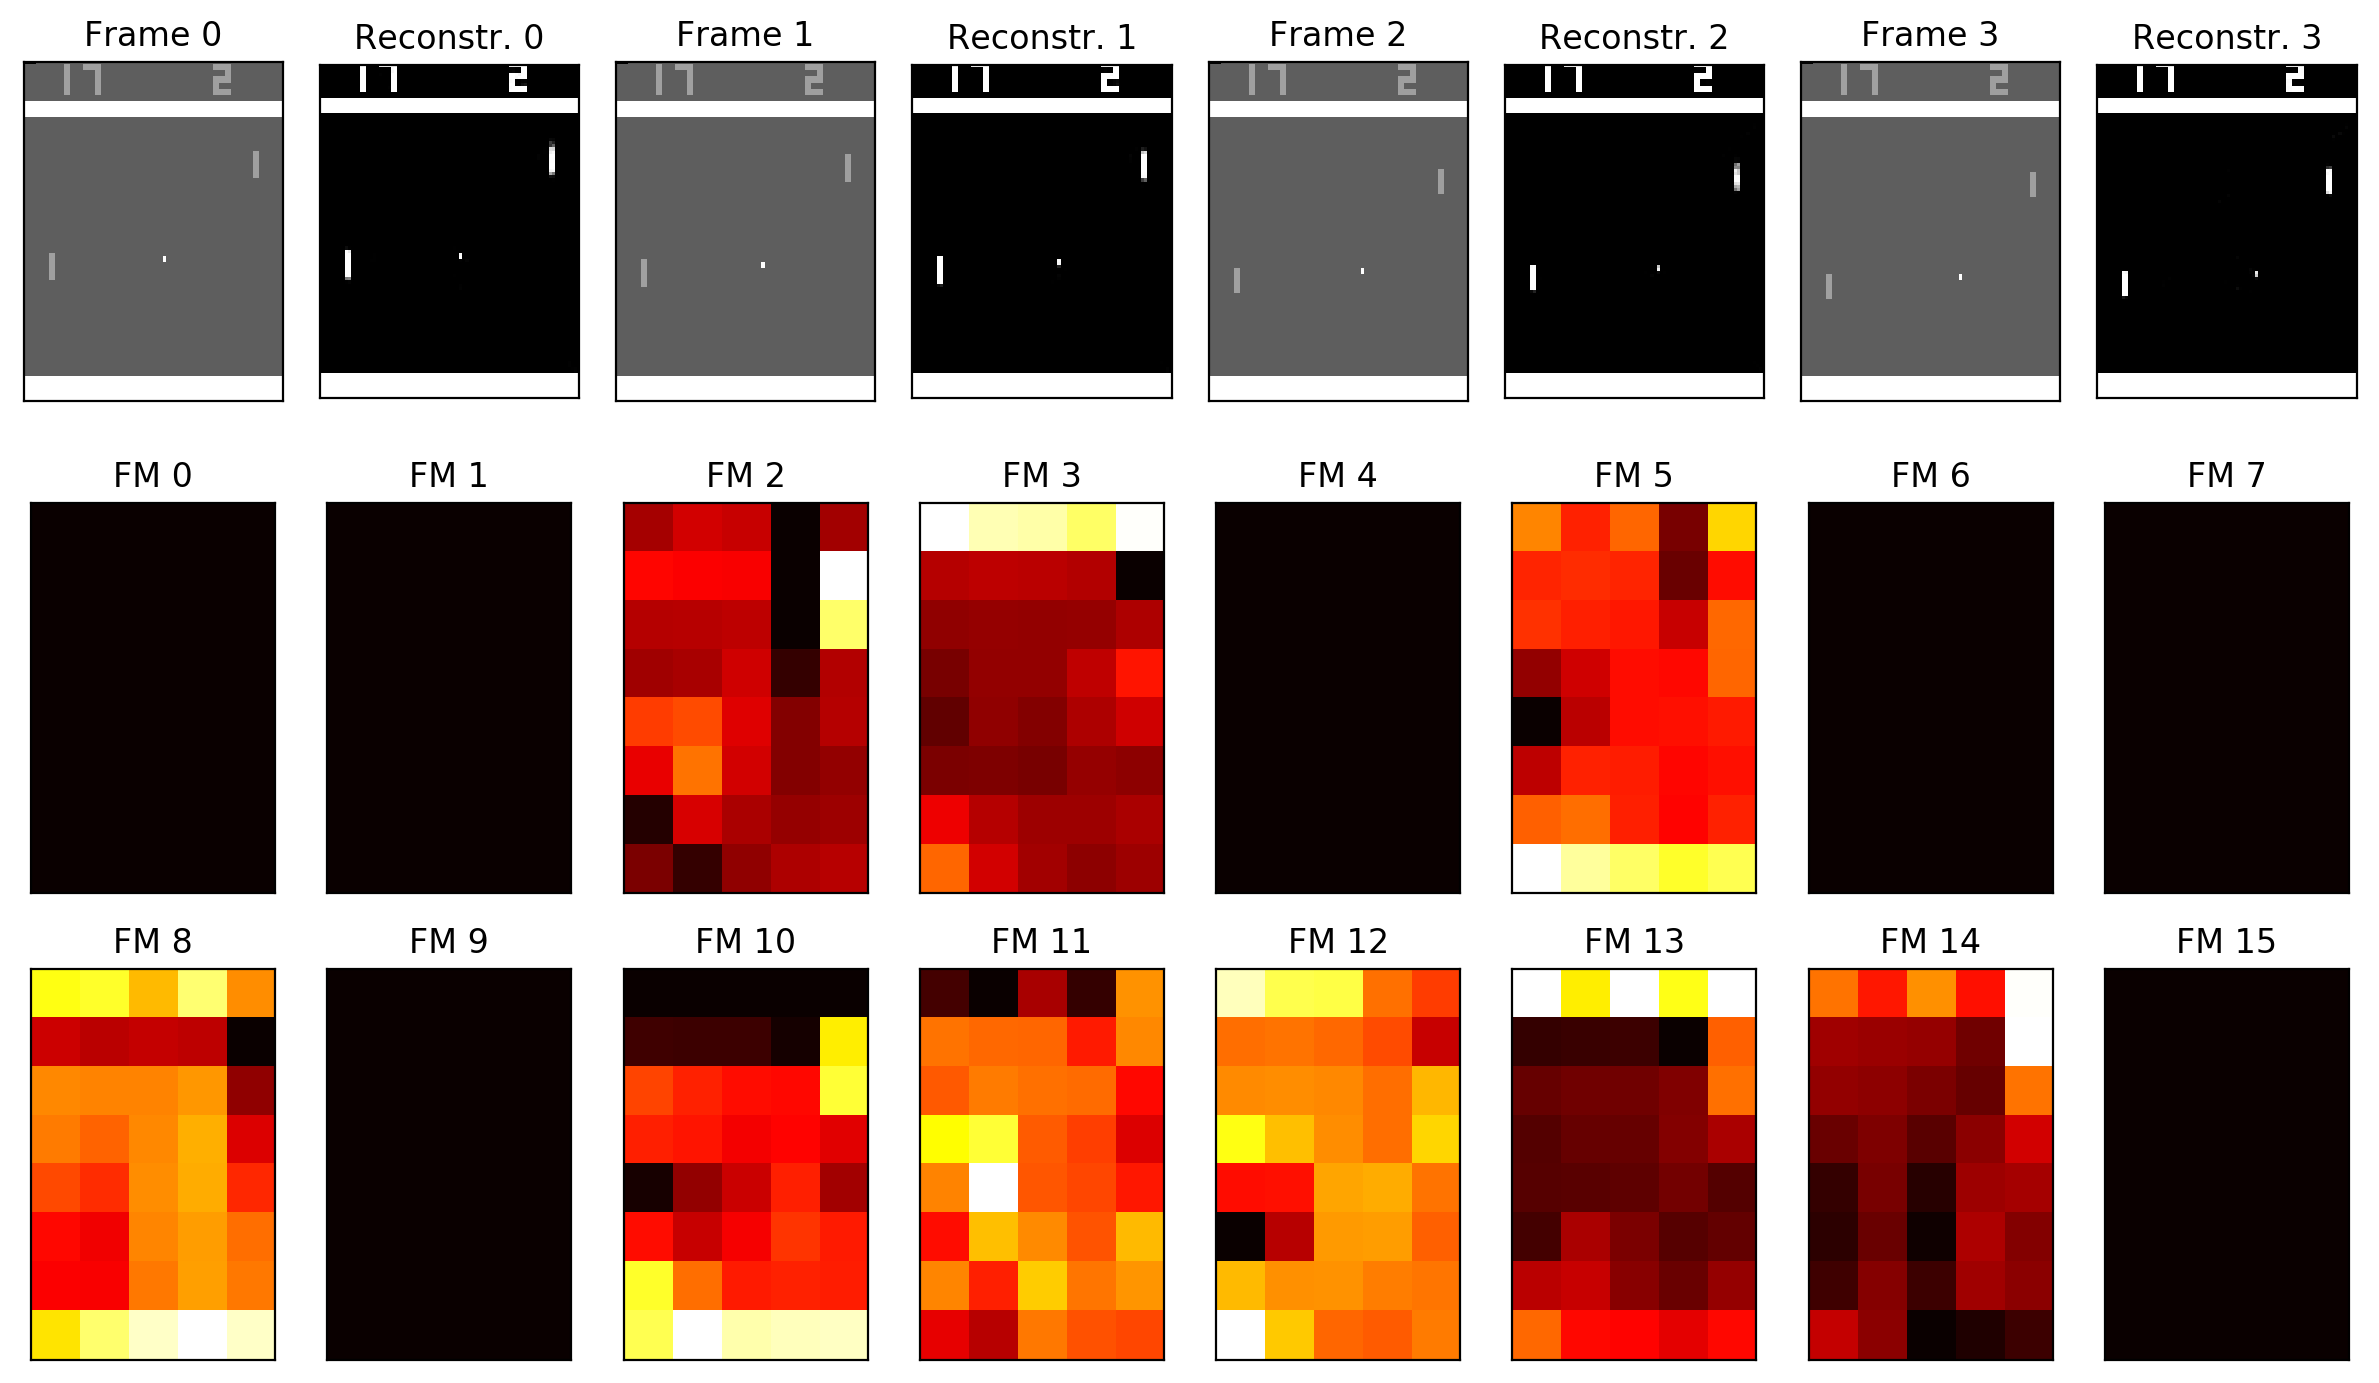
\includegraphics[width=\textwidth]{pictures/experiments/reconstr_pong}
    \centering
    \caption[AE reconstruction and feature maps on Pong]{AE reconstruction 
    and feature maps on Pong.}
    \label{f:P_reconstr}
\end{figure}
%
%
\begin{figure}
    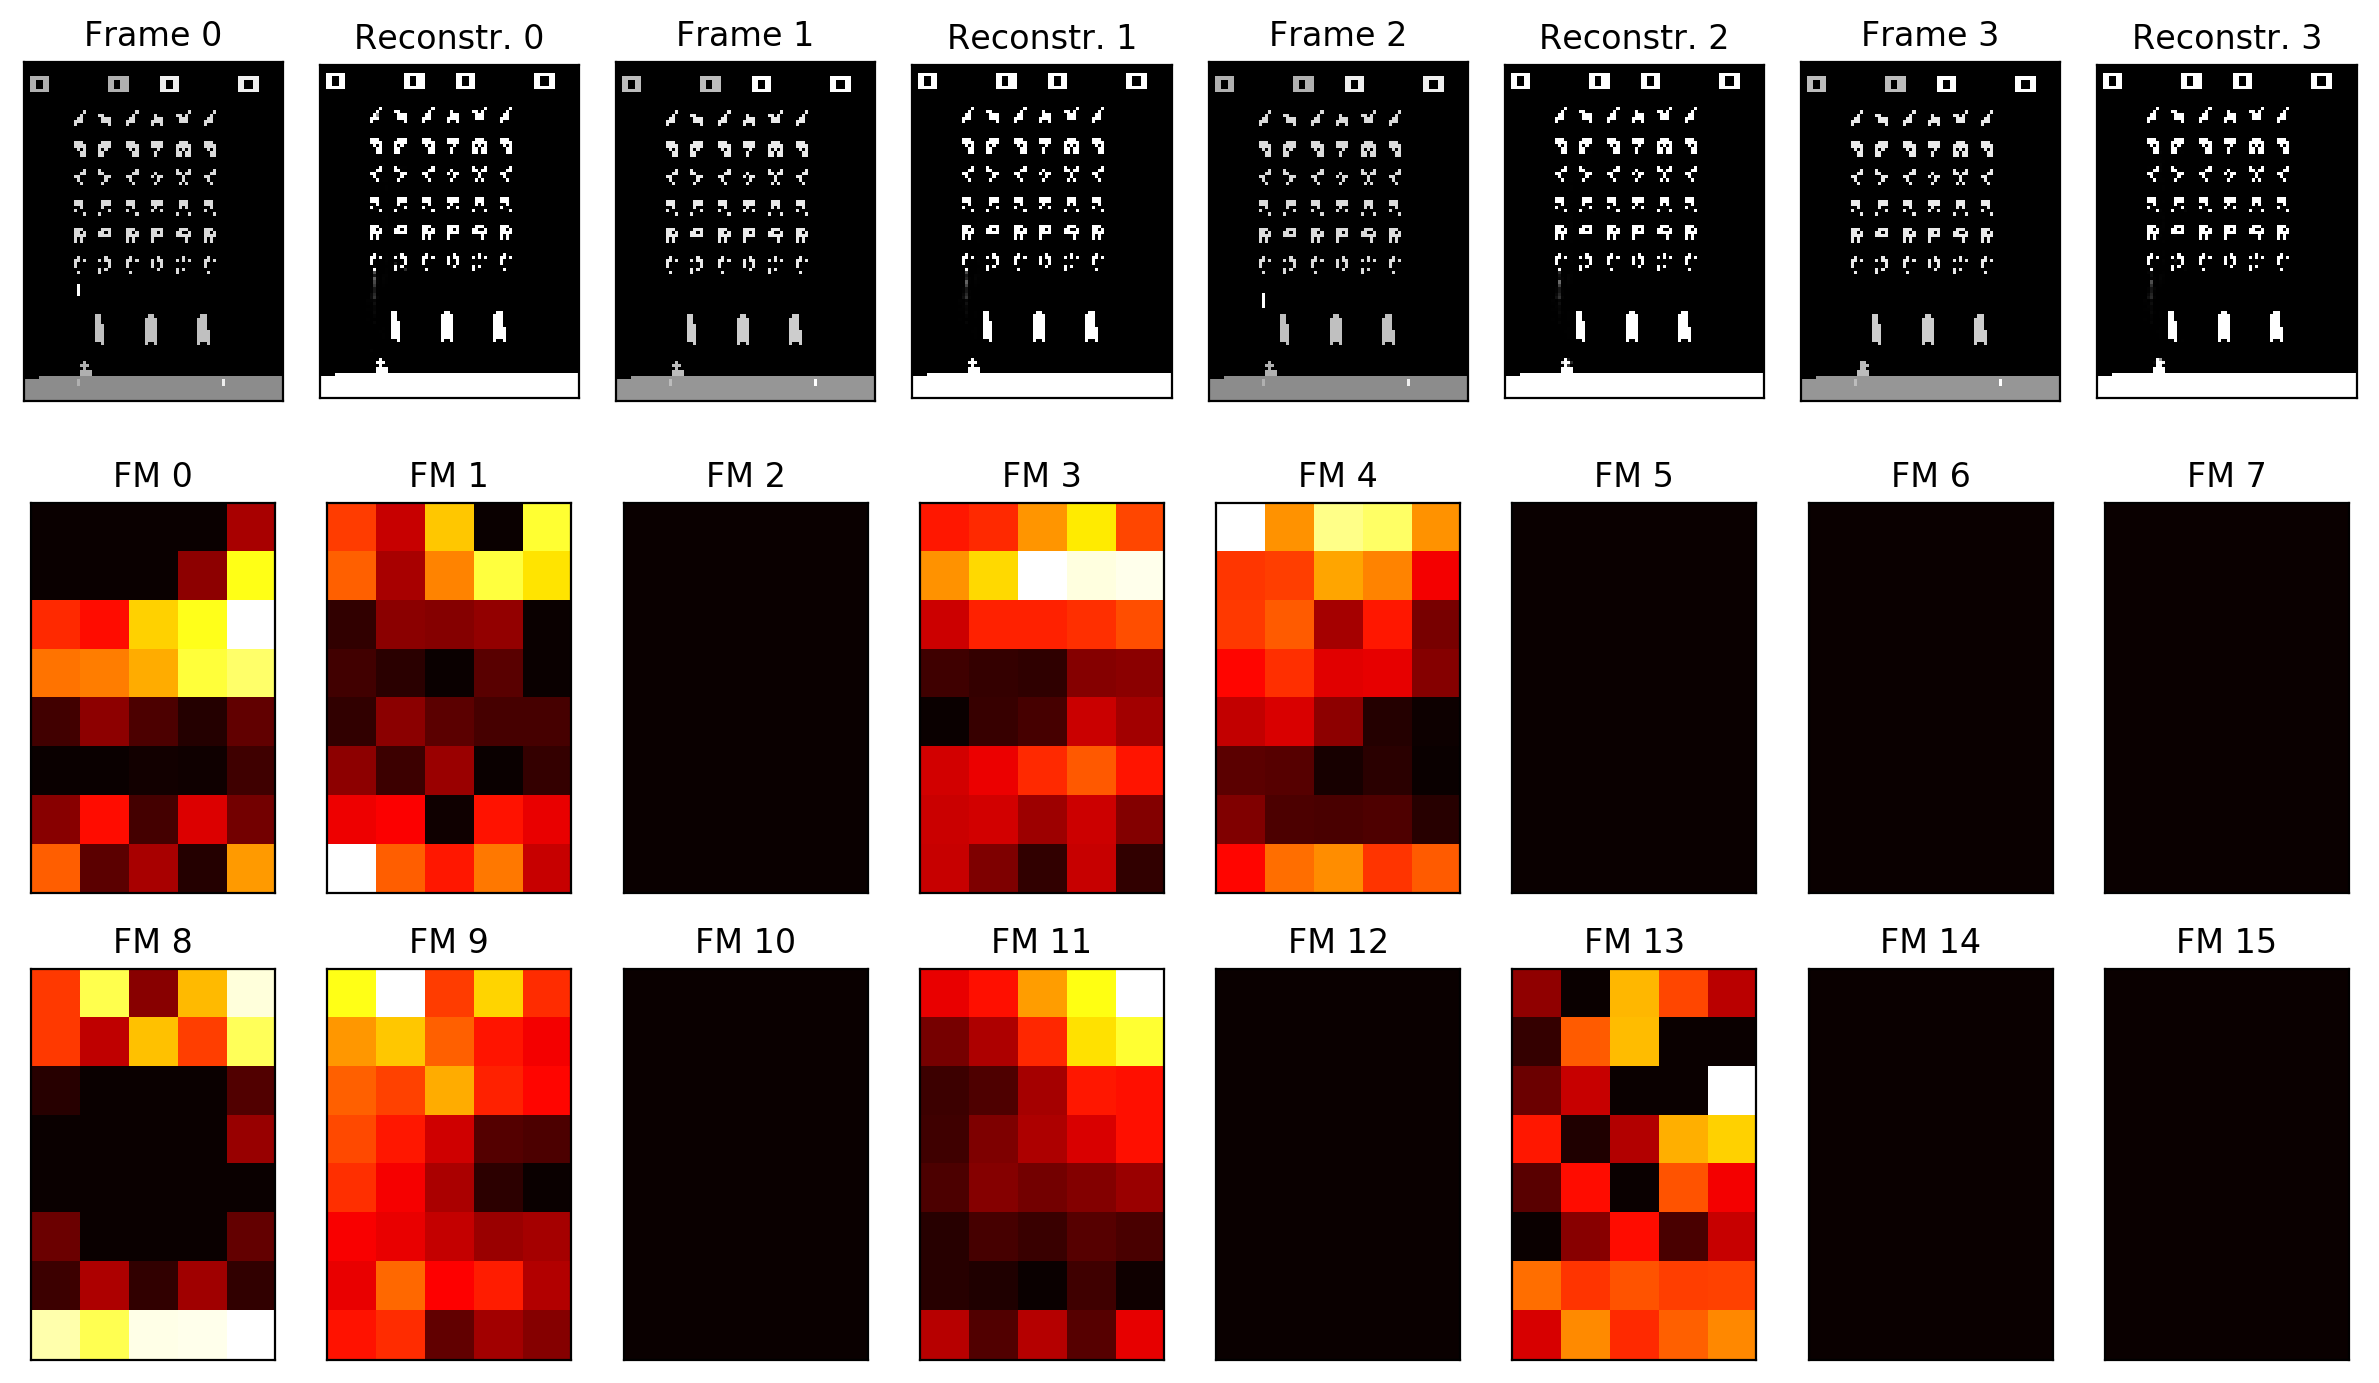
\includegraphics[width=\textwidth]{pictures/experiments/reconstr_space_invaders}
    \centering
    \caption[AE reconstruction and feature maps on Space Invaders]{AE reconstruction 
    and feature maps on Space Invaders. Note that the lower accuracy here translates
    to a poor definition in reconstructing moving elements like the player's
    character and projectiles.}
    \label{f:SI_reconstr}
\end{figure}
%

The most simple test that we run consisted in assessing the reconstruction loss
and accuracy on a held-out validation set (cf.\ Section \ref{s:ae_training_details}). 
We were able to achieve very high reconstruction accuracy in all environments, 
with no sensible differences between training sets collected under different 
exploration rates. In Table \ref{t:ae_training_precision} we report validation 
performance of the AE on fully random datasets of $\approx50000$ samples (see
also Figures \ref{f:BO_reconstr}, \ref{f:P_reconstr}, and \ref{f:SI_reconstr}).
%
\begin{table}
    \centering
    \begin{tabular}{l c c} 
	\hline
	Environment    & Val. loss        & Val. accuracy \\ 
	\hline 
	Breakout       & $\approx10^{-5}$ & $1.0$ \\
	Pong           & $\approx10^{-9}$ & $1.0$ \\
	Space Invaders & $\approx10^{-3}$ & $0.9987$ \\
	\hline
    \end{tabular}
    \caption[AE validation performance]{Validation performance of our AE on
	     fully random datasets of $\approx50000$ samples.}
    \label{t:ae_training_precision}
\end{table}
%
Less formally, a visual inspection of the reconstruction helped us in the early 
experimental phases and highlighted how even a small change in accuracy (in the
order of $10^{-3}$) could result in an incredibly noisy output.
At the same time, we also inspected the values and behaviors of the features 
maps produced by the encoder before flattening, by creating short animations (See
Figures \ref{f:BO_reconstr}, \ref{f:P_reconstr}, and \ref{f:SI_reconstr}) of 
how the activation values changed in a sequence of about a hundred states. 
This was done to make sure that the extracted features maps contained abstract
enough information (without excessive spatial correlation between the features),
but didn't give important insights.

In order to truly assess the compatibility of the extracted features 
with control problems, we trained a supervised model to learn the $Q$ 
approximation produced by DQN, using the extracted features (we call this 
a \textit{$\tilde{S}$-$Q$ test}). 
We used a training set composed of tuples $(ENC(s), q)$, where $s$ is a 
state from the environment, after the preprocessing described in Section 
\ref{s:atari_envs}, and $q$ is the $|A|$-dimensional estimate produced by DQN 
when it receives $s$ as input. Note that we could use the same input
for both networks, because the preprocessing that we perform on the observations 
before feeding a sample to the encoder (cf.\ Section \ref{s:atari_envs}) 
are basically the same that are applied to the inputs for DQN. To account for 
the slight different preprocessing, we computed $q$ before applying the 
transformations which are unique to our preprocessing, namely the binarization 
and cropping. 
For each environment, we used the best performing DQN described in Section 
\ref{s:exp_baseline} to produce the targets, and we sample $\approx50000$ states
from the same dataset on which the AE was trained.
To learn the $Q$ approximation, we used the same Extra-Trees model and 
hyperparameters that we use for FQI (See Tables \ref{t:FQI_tree_params} and
\ref{t:FQI_extra_params}), to ensure that the configuration itself was 
adequate to describe the nonlinear relations between the features and the 
action-value function at convergence of FQI. 
This was done by simply fitting the model on the $(ENC(s), q)$ pairs, and 
evaluating the $R^2$ score (cf.\ Definition \eqref{e:R2}) and \textit{Mean 
Squared Error} (MSE) of the predictions on a held-out validation set of roughly 
$5\%$ of the training samples.
We report the results of these tests, run on datasets collected with different
values of $\varepsilon$ at different iterations of our full algorithm, in 
Table \ref{t:FQ_tests}.
As seen in figure \ref{f:FQ_test_all_three}, the extracted features are suitable for 
describing the $Q$ function learned by DQN with a good degree if precision, and 
constitute an adequate base for our whole approach. 
%
\begin{table}
    \centering
    \begin{tabular}{l c c c} 
	\hline
	Environment    & $\varepsilon$ & $R^2$   & MSE \\ 
	\hline 
	Breakout       & $1.0$         & $ $     & $ $ \\
	Pong 	       & $1.0$         & $0.945$ & $0.0167$ \\
	Space Invaders & $ $           & $ $     & $ $ \\
	\hline
    \end{tabular}
    \caption[Results of $\tilde{S}$-$Q$ mapping experiment]{Results of the 
	     $\tilde{S}$-$Q$ mapping experiment with different exploration rates
	     to collect the datasets.}
    \label{t:FQ_tests}
\end{table}
%
%
\begin{figure}
    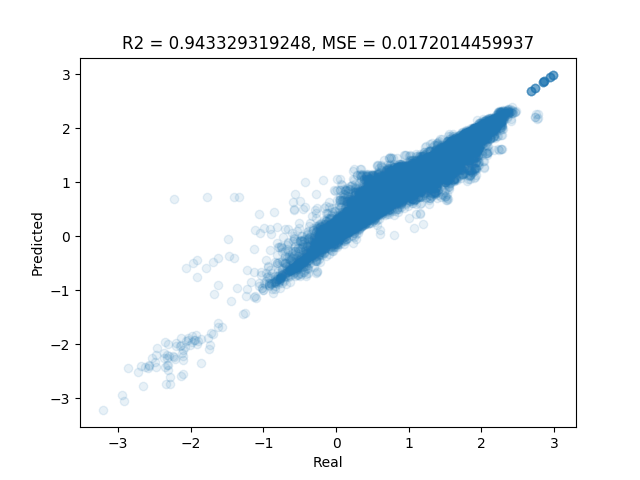
\includegraphics[width=\textwidth]{pictures/experiments/FQ_test_pong}
    \centering
    \caption[Predictions of $\tilde{S}$-$Q$ mapping experiment]{Values predicted 
	     by the supervised model in the $\tilde{S}$-$Q$ test vs.\ real values
	     predicted by DQN. Note that the $|A|$-dimensional estimate is 
	     flattened and treated as a sequence of $|A|$ predictions in order to
	     plot it.}
    \label{f:FQ_test_breakout}
\end{figure}
%
%
\begin{figure}
    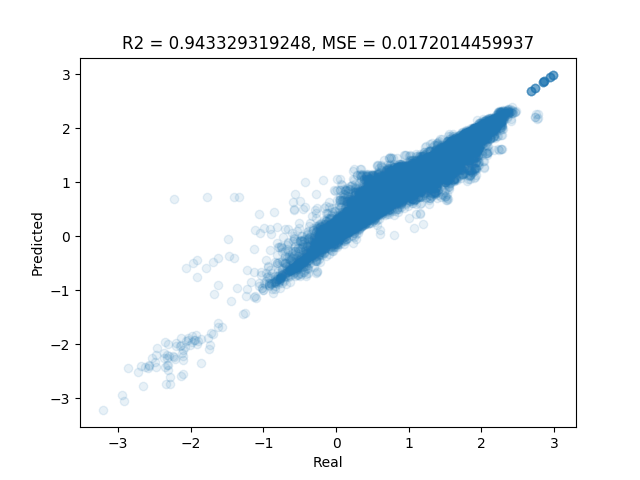
\includegraphics[width=\textwidth]{pictures/experiments/FQ_test_pong}
    \centering
    \caption[Predictions of $\tilde{S}$-$Q$ mapping experiment]{Values predicted 
	     by the supervised model in the $\tilde{S}$-$Q$ test vs.\ real values
	     predicted by DQN. Note that the $|A|$-dimensional estimate is 
	     flattened and treated as a sequence of $|A|$ predictions in order to
	     plot it.}
    \label{f:FQ_test_pong}
\end{figure}
%
%
\begin{figure}
    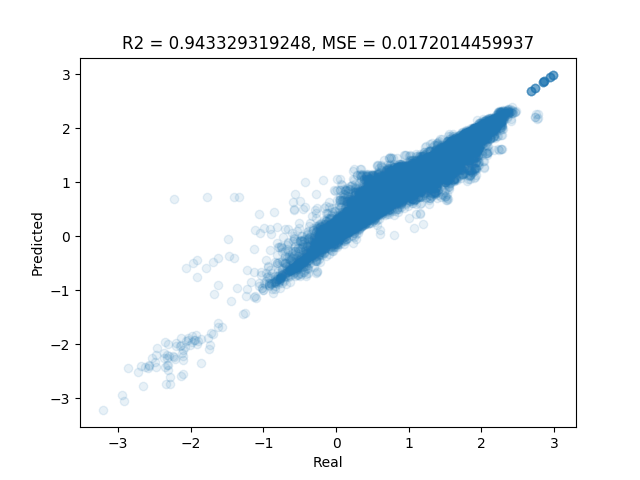
\includegraphics[width=\textwidth]{pictures/experiments/FQ_test_pong}
    \centering
    \caption[Predictions of $\tilde{S}$-$Q$ mapping experiment]{Values predicted 
	     by the supervised model in the $\tilde{S}$-$Q$ test vs.\ real values
	     predicted by DQN. Note that the $|A|$-dimensional estimate is 
	     flattened and treated as a sequence of $|A|$ predictions in order to
	     plot it.}
    \label{f:FQ_test_space_invaders}
\end{figure}
%

\section{Recursive Feature Selection}
The main purpose of RFS in our learning pipeline is to provide a fast forward 
propagation of the AE at control time, by keeping only the AE weights that are 
essential for the representation. 
The runtime of RFS, however, is the longest amongst the three main components, 
taking up to a week to complete and extending the runtime of the full algorithm
to a point where it becomes unfeasible. We therefore had to ignore the RFS 
part of the training steps during most of our experiments, resorting to only
running it once per environment using a dataset collected under a fully random 
policy and an AE trained on the same dataset (as if we were running the 
selection at the first step of the main procedure). 
At the same time, we found it appropriate to run another simple feature 
selection technique which consisted in only keeping those features with nonzero 
variance (NZV), in order to simplify our feature space without losing 
information. 
We found that RFS reduced the representation by up to $60\%$ with respect to NZV,
which indicates that the AE does indeed extract a great deal of redundancy that
can be ignored for control purposes. 
In Figures \ref{f:rfs_tree_breakout}, \ref{f:rfs_tree_pong} and 
\ref{f:rfs_tree_space_invaders} we show the graphical representation of the 
feature selection as dependency trees.
%
\begin{table}
    \centering
    \begin{tabular}{l c c c} 
	\hline
	Environment    & Original & NZV   & RFS \\ 
	\hline 
	Breakout       & $640$    & $599$ & $ $ \\
	Pong           & $640$    & $585$ & $245$ \\
	Space Invaders & $640$    & $320$ & $ $ \\
	\hline
    \end{tabular}
    \caption[Feature selection results]{Number of features kept by the two 
	     feature selection techniques that we used in our experiments, run 
	     on datasets of $100000$ samples collected under a fully random 
	     policy.}
    \label{t:RFS_results}
\end{table}
%
%
\begin{figure}
    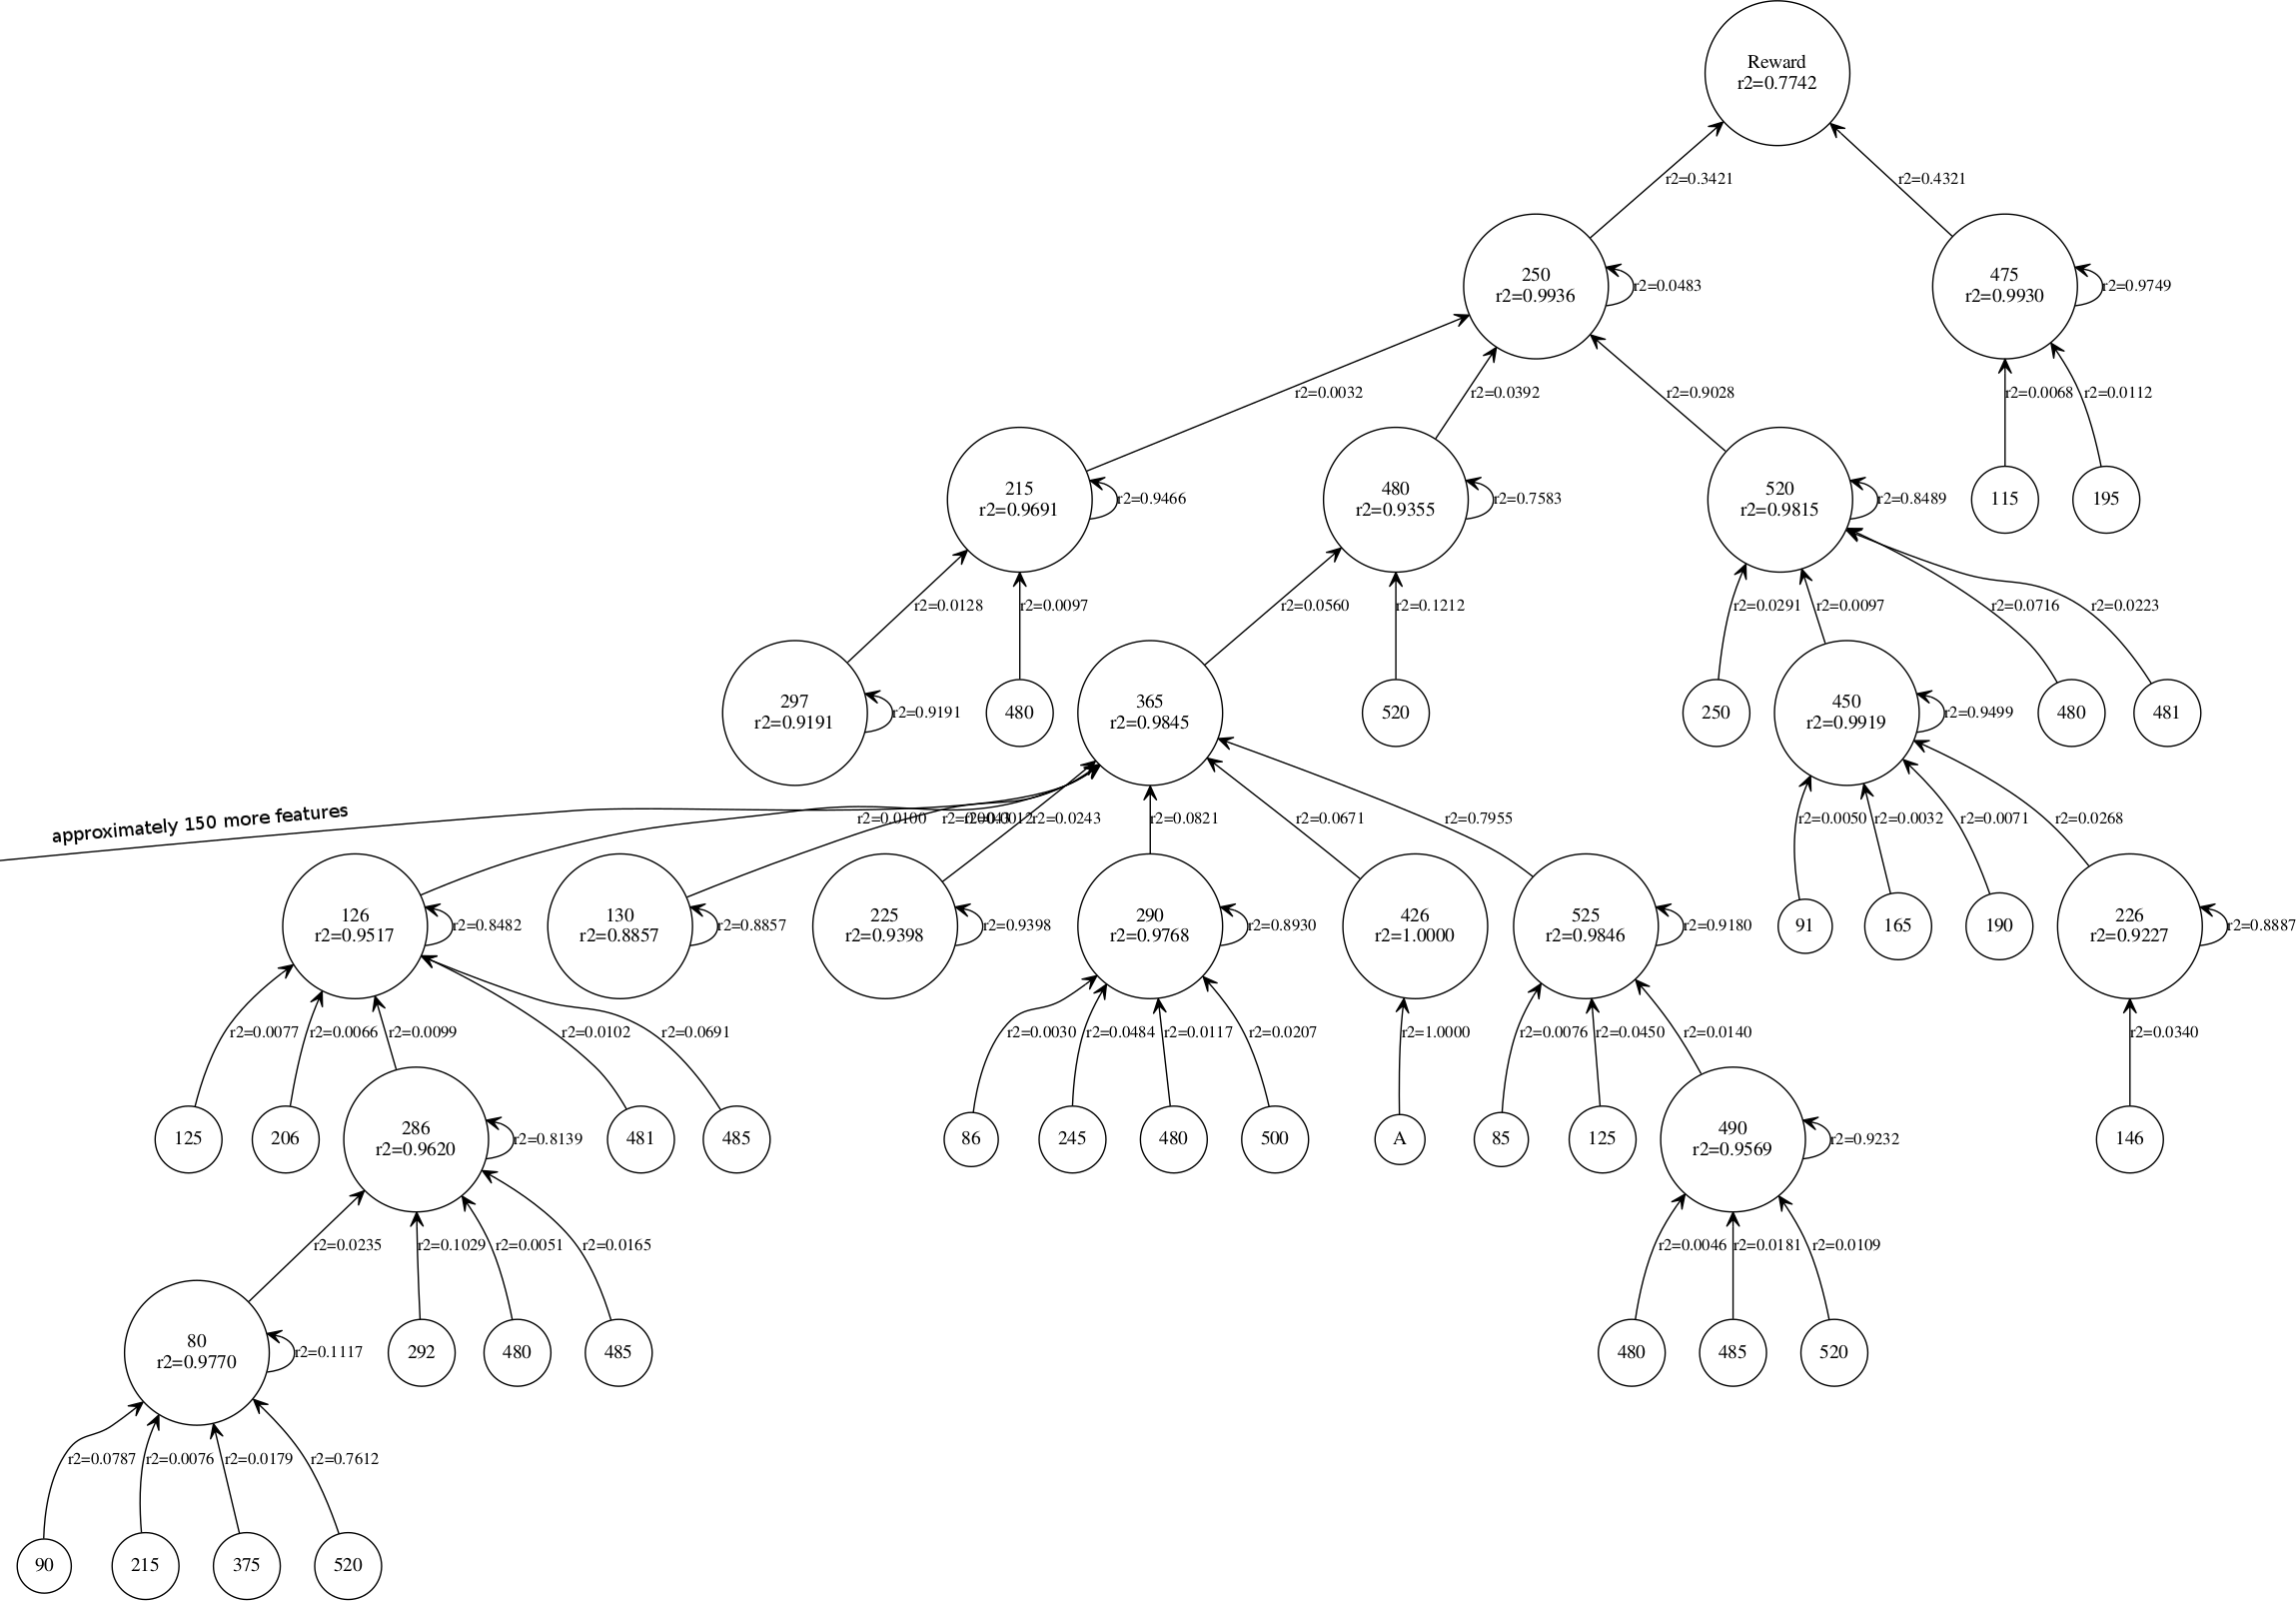
\includegraphics[width=\textwidth]{pictures/experiments/rfs_tree_top_pong}
    \centering
    \caption[RFS dependency tree in Breakout]{RFS dependency tree in Breakout 
	     (showing only topmost nodes).}
    \label{f:rfs_tree_breakout}
\end{figure}
%
%
\begin{figure}
    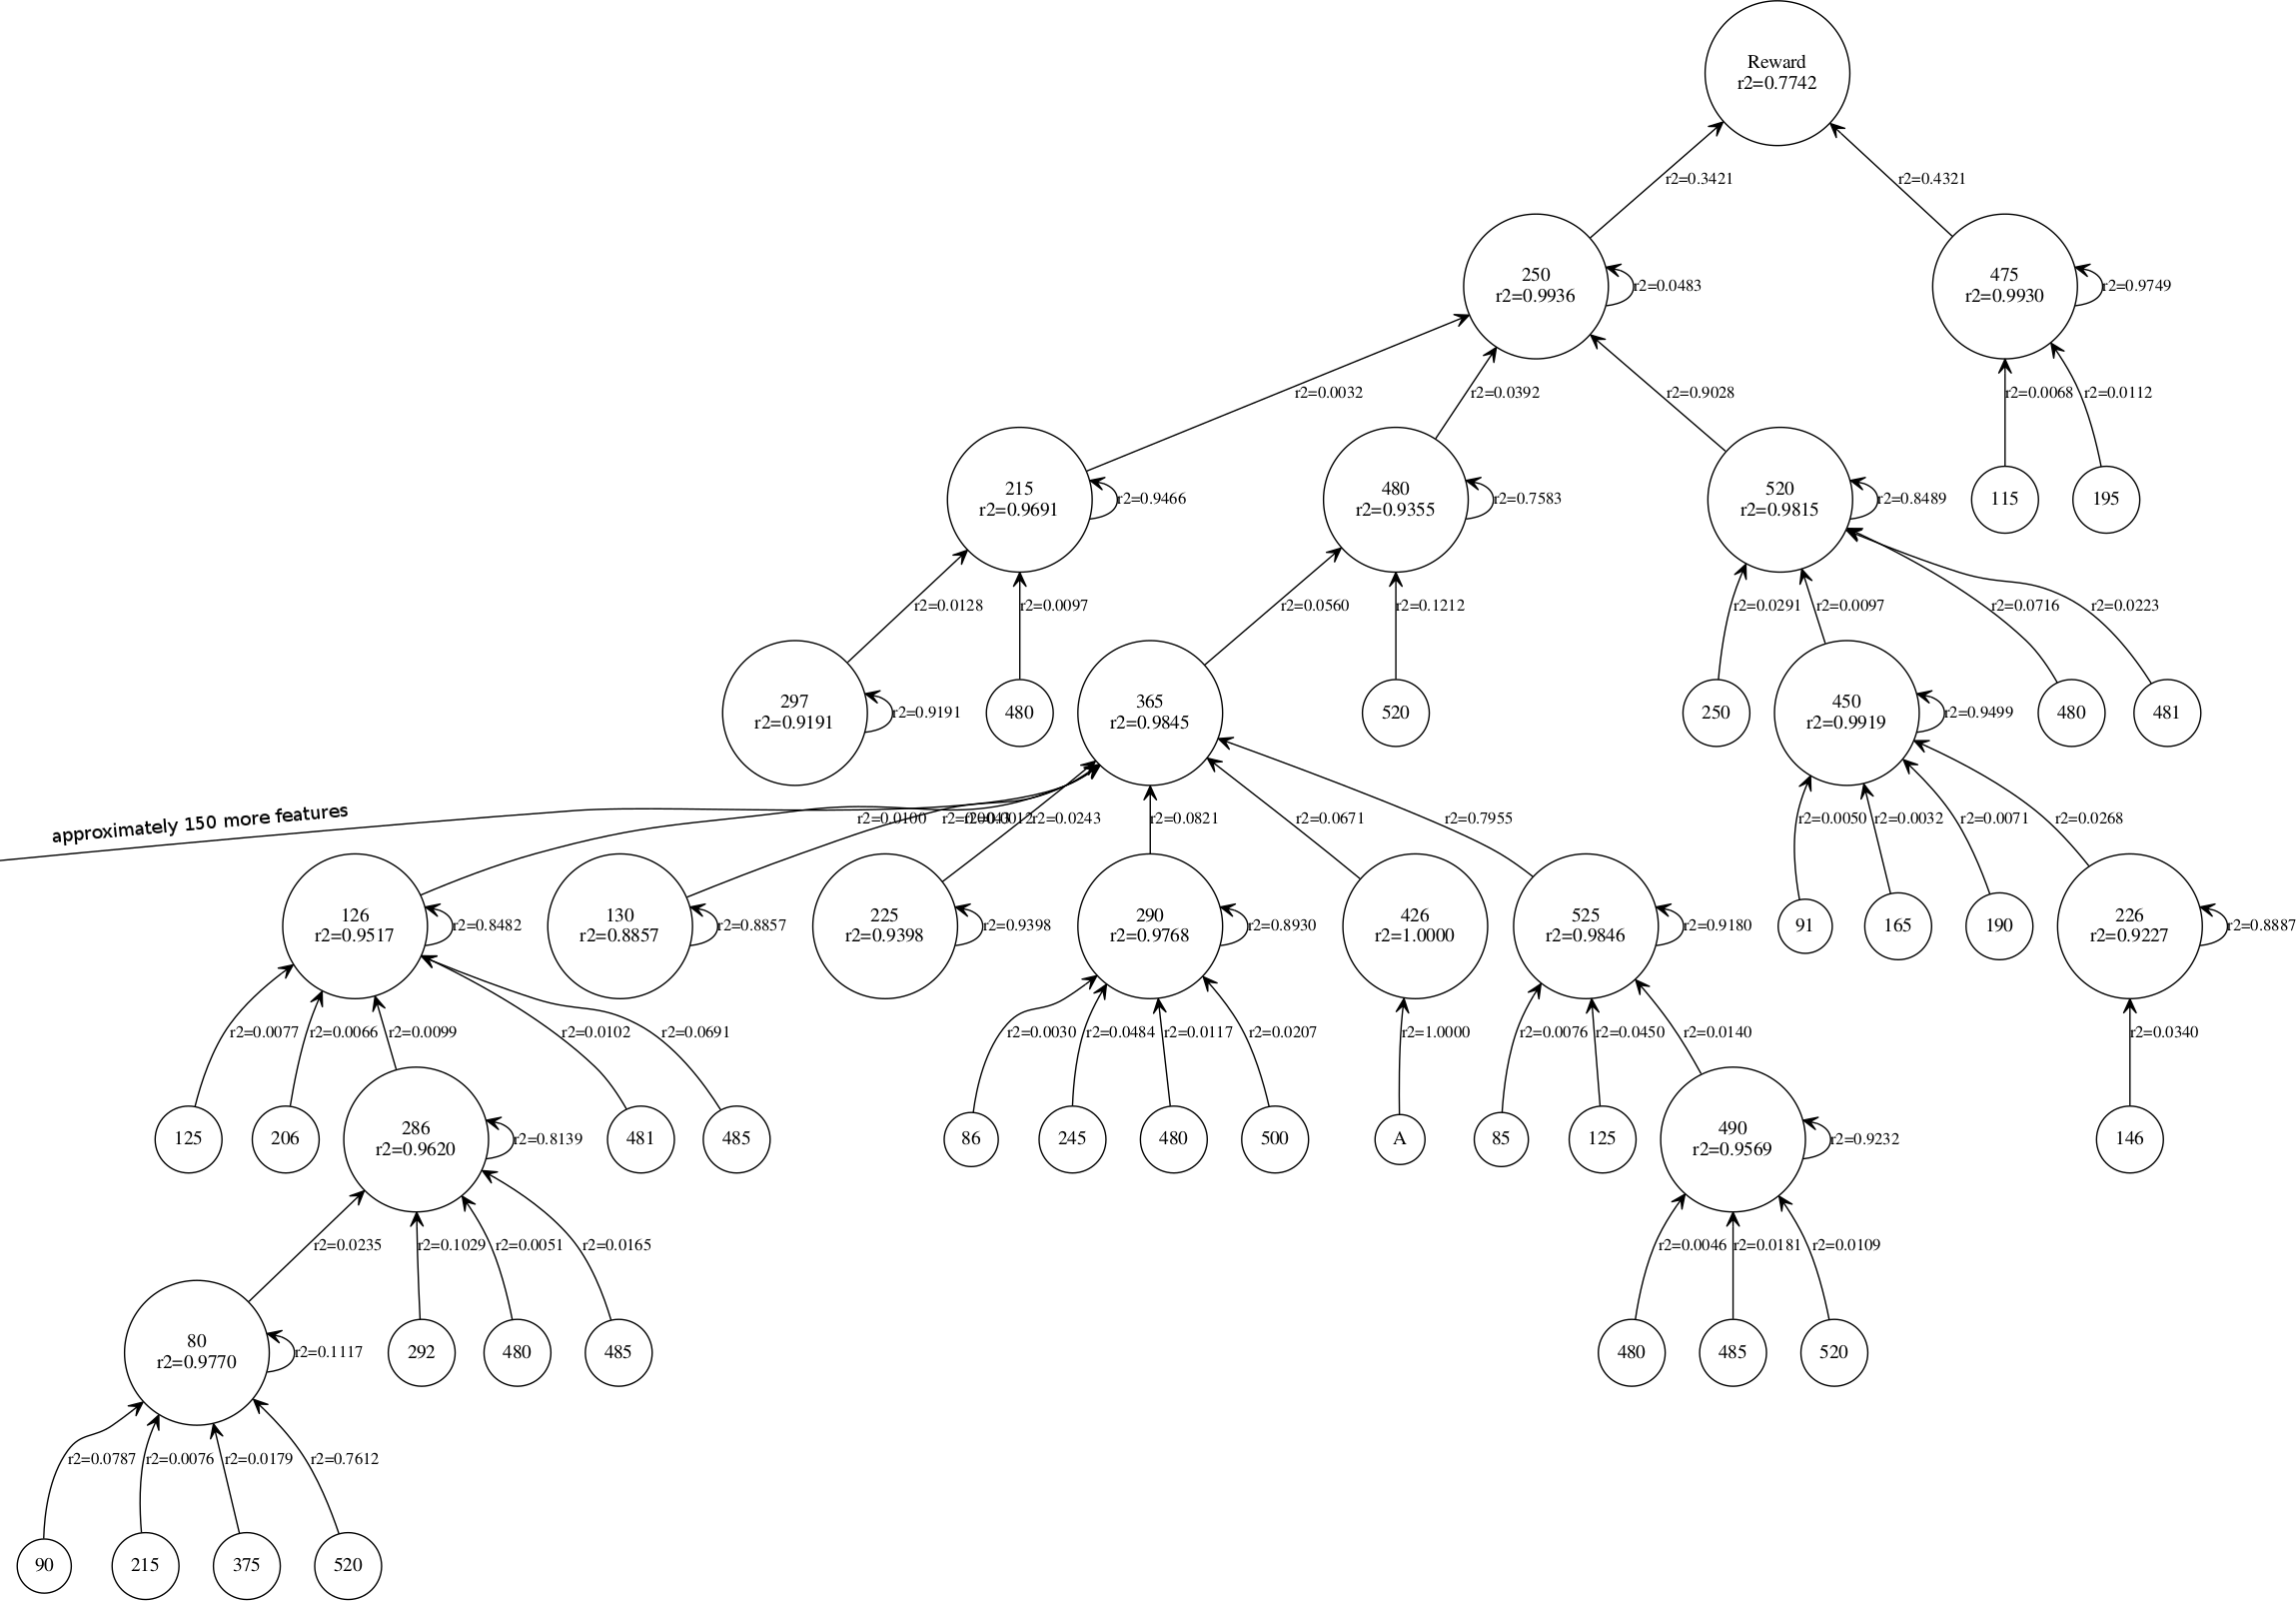
\includegraphics[width=\textwidth]{pictures/experiments/rfs_tree_top_pong}
    \centering
    \caption[RFS dependency tree in Pong]{RFS dependency tree in Pong 
	     (showing only topmost 50 nodes).}
    \label{f:rfs_tree_pong}
\end{figure}
%
%
\begin{figure}
    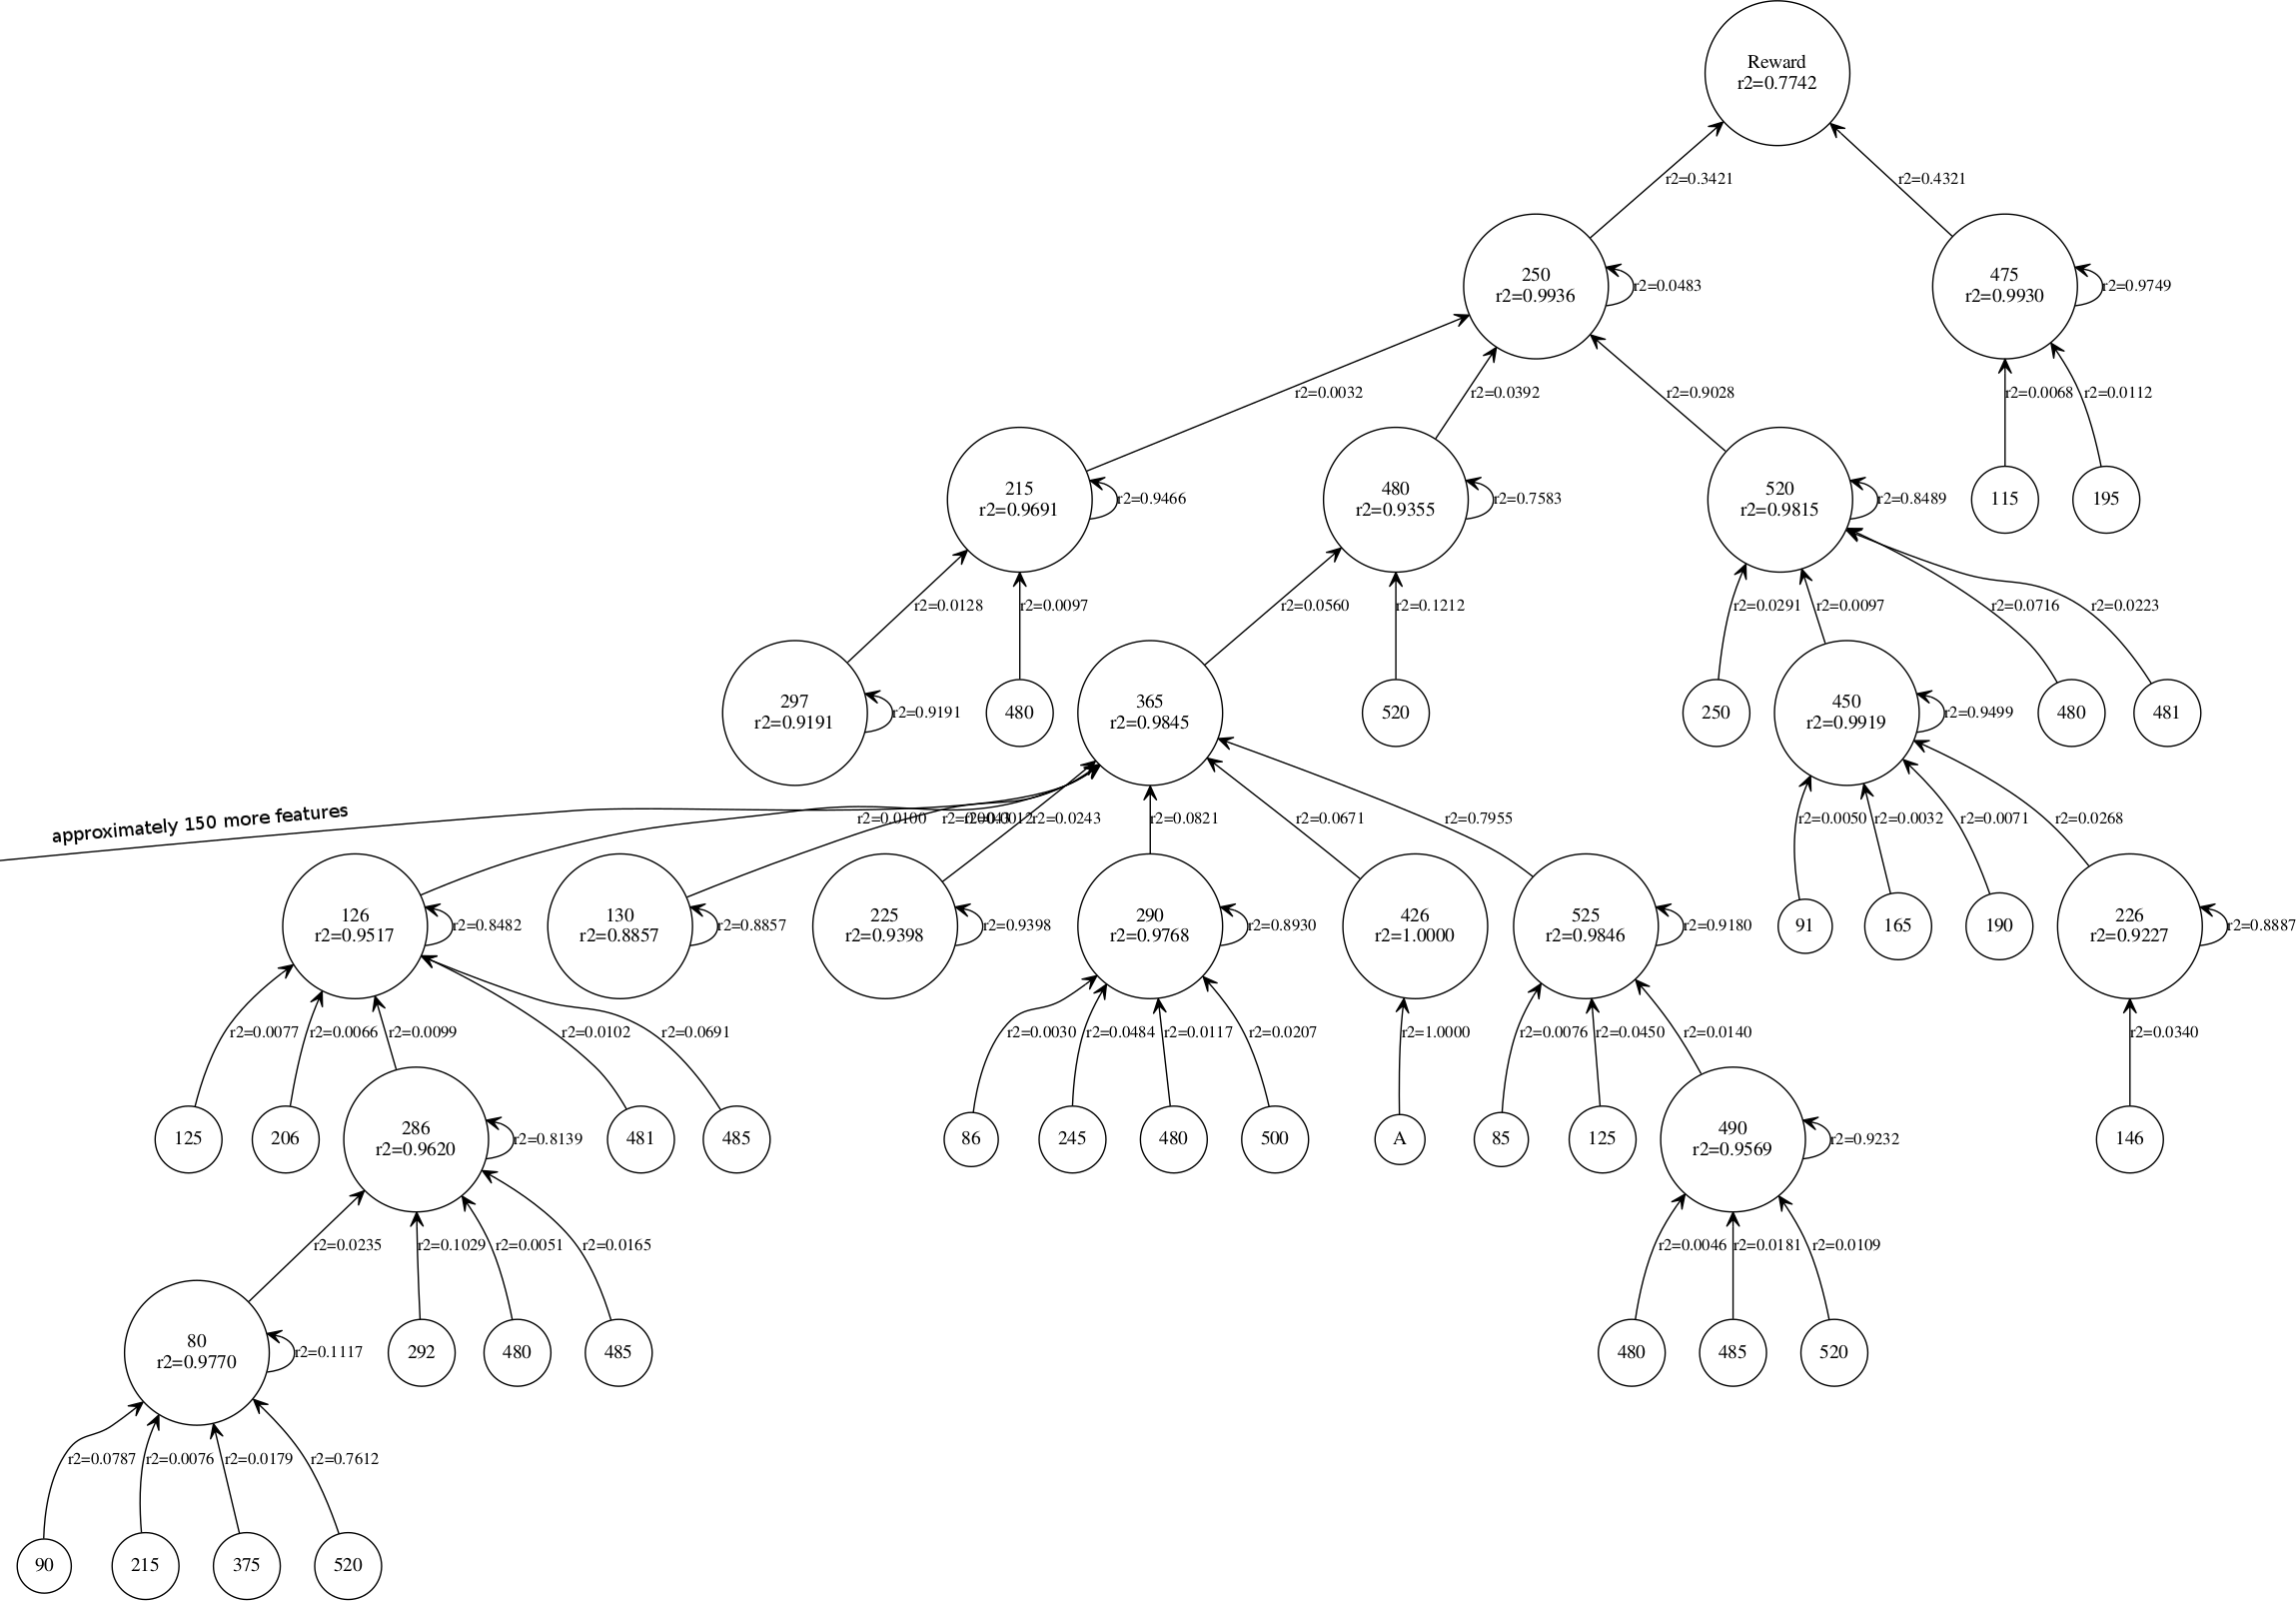
\includegraphics[width=\textwidth]{pictures/experiments/rfs_tree_top_pong}
    \centering
    \caption[RFS dependency tree in Space Invaders]{RFS dependency tree in Space 
	     Invaders (showing only topmost nodes).}
    \label{f:rfs_tree_space_invaders}
\end{figure}
%
\section{Fitted Q-Iteration}

% Baseline
    % Breakout, Pong, Space Invaders, Other (with info on specific envs?)
    % Baseline with DQN
	% BO.........................................................[GOT][DONE]
	% P..........................................................[GOT][DONE]
	% SI.........................................................[GOT][DONE]
	% Other......................................................[][]

% AE
    % Reconstructions + Feature maps plots
	% BO.........................................................[GOT][DONE]
	% P..........................................................[GOT][DONE] (Missing .gif for slides)
	% SI.........................................................[GOT][DONE]
	% Other......................................................[][]
    % FQ Test + FQ Score
	% BO.........................................................[][]
	% P..........................................................[][]
	% SI.........................................................[][]
	% Other......................................................[][]

% RFS
    % Whatever envs you have
    % Whatever feature analysis you want
    % Mention NZV selection to speed up training
	% BO.........................................................[][]
	% P..........................................................[GOT][]
	% SI.........................................................[][]
	% Other......................................................[][]

% FQI
    % Comparison with DQN at same number of frames...................[][]
    % BO.............................................................[][]
    % P..............................................................[][]
    % SI.............................................................[][]
    % Other..........................................................[][]
    




